\begin{comment}
Template vir elke funksie
    \paragraph{Funksie naam}
			\begin{description}
			    \item{\textbf{Priority}:} %watter prioriteit dit het: Critical, Important of Nic-to-have
			    \item{\textbf{Service Contract}:}% Wat dit doen
			    \item{\textbf{Pre-conditions}:}%wat moet waar wees voor die funksie sy ding kan doen
    			    \begin{itemize}
    			        \item %precondition 1
    			        \item %precondition 2
    			    \end{itemize}
			    \item{\textbf{Post-conditions}:} % wat moet waar wees na die funksie sy ding gedoen het
    			    \begin{itemize}
    			    \item %post condition 1
    			    \item %post condition2
    			    \end{itemize}
			\end{description}
\end{comment}






\subsection{Node}
    \subsubsection{Scope:} 
    \begin{itemize}
    \item The node is connected to the gateway with a serial connection.
    \item The node uses NFC to communicate with the Protection App on the phone.
    \item When the phone is scanned, it sends the device id of the phone to the node. The node then sends it to the gateway to verify if the user has access to the meeting. When the gateway replies with the results of the verification, the node turns the lights the appropriate colour, decides if the door must be unlocked and sends feedback to the phone.
    
    \end{itemize} 
    
    \begin{figure}[H]
 			 \centering
			  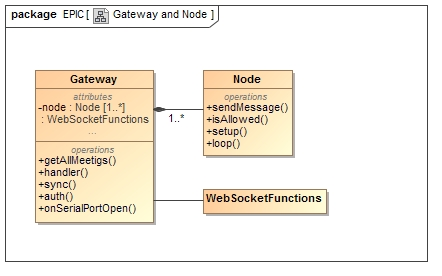
\includegraphics[width=12cm]{GatewayAndNodeClass}
		 	 \caption{A Class Diagram of the Gateway and Node}
		\end{figure}
		
    \subsubsection{Functionality}
        \paragraph{isAllowed}
			\begin{description}
			    \item{\textbf{Priority}:} Critical%watter prioriteit dit het: Critical, Important of Nic-to-have
			    \item{\textbf{Service Contract}:} Sends the device ID to the Gateway and waits until it receives the results on whether or not to allow the user in.% Wat dit doen
			    \item{\textbf{Pre-conditions}:}%wat moet waar wees voor die funksie sy ding kan doen
    			    \begin{itemize}
    			        \item The users' phone should be on the Node.
    			        \item The Protection App should have sent the device ID.
    			    \end{itemize}
			    \item{\textbf{Post-conditions}:} % wat moet waar wees na die funksie sy ding gedoen het
    			    \begin{itemize}
    			        \item The Gateway should have sent a reply.
    			        \item The sendMessage function should be called.
    			    \end{itemize}
			\end{description}

        \paragraph{sendMessage}
			\begin{description}
			    \item{\textbf{Priority}:} Critical%watter prioriteit dit het: Critical, Important of Nic-to-have
			    \item{\textbf{Service Contract}:} This function adapts the results to the correct format that the Protection App is expecting, and then broadcasts it via NFC to the phone. It also calls the setColor function with the appropriate values and calls the openDoor function if the user is allowed in the meeting.
			    \item{\textbf{Pre-conditions}:}%wat moet waar wees voor die funksie sy ding kan doen
    			    \begin{itemize}
    			        \item The results from the Gateway should be received.
    			        \item The users' phone should still be on the Node.
    			    \end{itemize}
			    \item{\textbf{Post-conditions}:} % wat moet waar wees na die funksie sy ding gedoen het
    			    \begin{itemize}
    			        \item The Protection App should have received the results.
    			        \item The lights should reflect the colour of the results.
    			        \item The door should be unlocked if the lights turned green.
    			    \end{itemize}
			\end{description}
		
        \paragraph{setColor}
			\begin{description}
			    \item{\textbf{Priority}:} Important%watter prioriteit dit het: Critical, Important of Nic-to-have
			    \item{\textbf{Service Contract}:} This function receives an RGB colour value and sets the lights to turn that colour. 
			    \item{\textbf{Pre-conditions}:}%wat moet waar wees voor die funksie sy ding kan doen
    			    \begin{itemize}
    			        \item The lights should have power.
    			    \end{itemize}
			    \item{\textbf{Post-conditions}:} % wat moet waar wees na die funksie sy ding gedoen het
    			    \begin{itemize}
    			        \item The lights should be the desired colour.
    			    \end{itemize}
			\end{description}
			
		\paragraph{openDoor}
			\begin{description}
			    \item{\textbf{Priority}:} Nice-to-have%watter prioriteit dit het: Critical, Important of Nic-to-have
			    \item{\textbf{Service Contract}:} This function unlocks the door temporarily so that the user can enter the meeting room.
			    \item{\textbf{Pre-conditions}:}%wat moet waar wees voor die funksie sy ding kan doen
    			    \begin{itemize}
    			        \item The door should be locked.
    			        \item The user must be in front of the door.
    			    \end{itemize}
			    \item{\textbf{Post-conditions}:} % wat moet waar wees na die funksie sy ding gedoen het
    			    \begin{itemize}
    			        \item The door should be locked again.
    			        \item The user must be on the other side of the door.
    			    \end{itemize}
			\end{description}
			
		\paragraph{waiting}
			\begin{description}
			    \item{\textbf{Priority}:} Important%watter prioriteit dit het: Critical, Important of Nic-to-have
			    \item{\textbf{Service Contract}:} Runs the lights through a sequence and delays the loop function a bit. 
			    \item{\textbf{Pre-conditions}:}%wat moet waar wees voor die funksie sy ding kan doen
    			    \begin{itemize}
    			        \item None
    			    \end{itemize}
			    \item{\textbf{Post-conditions}:} % wat moet waar wees na die funksie sy ding gedoen het
    			    \begin{itemize}
    			        \item None
    			    \end{itemize}
			\end{description}
			
		\paragraph{setup}
			\begin{description}
			    \item{\textbf{Priority}:} Critical%watter prioriteit dit het: Critical, Important of Nic-to-have
			    \item{\textbf{Service Contract}:} Initialises the necessary variables and objects and starts the loop function. 
			    \item{\textbf{Pre-conditions}:}%wat moet waar wees voor die funksie sy ding kan doen
    			    \begin{itemize}
    			        \item The Node should be plugged in.
    			    \end{itemize}
			    \item{\textbf{Post-conditions}:} % wat moet waar wees na die funksie sy ding gedoen het
    			    \begin{itemize}
    			        \item The necessary variables and objects should be created in memory.
    			        \item The loop function should have been called.
    			    \end{itemize}
			\end{description}


		 \paragraph{loop}
			\begin{description}
			    \item{\textbf{Priority}:} Critical%watter prioriteit dit het: Critical, Important of Nic-to-have
			    \item{\textbf{Service Contract}:} Gets automatically called over and over like an infinite loop. Each time this function executes it calls the waiting function and then checks for input from the NFC board. When a valid identifier is received, it calls the sendMessage function with the results from the isAllowed function.
			    \item{\textbf{Pre-conditions}:}%wat moet waar wees voor die funksie sy ding kan doen
    			    \begin{itemize}
    			        \item The setup function should have succesfuly completed.
    			    \end{itemize}
			    \item{\textbf{Post-conditions}:} % wat moet waar wees na die funksie sy ding gedoen het
    			    \begin{itemize}
    			        \item Either Nothing should have happened,
    			        \item or the user should have his access granted or denied.
    			    \end{itemize}
			\end{description}

		